%Template by Mark Jervelund - 2015 - mjerv15@student.sdu.dk

\documentclass[a4paper,10pt,titlepage]{report}

\usepackage[utf8]{inputenc}
\usepackage[T1]{fontenc}
\usepackage[english]{babel}
\usepackage{amssymb}
\usepackage{amsmath}
\usepackage{amsthm}
\usepackage{graphicx}
\usepackage{fancyhdr}
\usepackage{lastpage}
\usepackage{listings}
\usepackage{algorithm}
\usepackage{algpseudocode}
\usepackage[document]{ragged2e}
\usepackage[margin=1in]{geometry}
\usepackage{color}
\usepackage{datenumber}
\usepackage{venndiagram}
\usepackage{chngcntr}
\usepackage[utf8]{inputenc}
\usepackage[english]{babel}
\usepackage{amssymb,amsmath,amsthm}
\usepackage{mathtools}
\newtheorem{theorem}{Theorem}

\usepackage{mathtools} % Bonus
\DeclarePairedDelimiter\norm\lVert\rVert
\setdatetoday
\addtocounter{datenumber}{0} %date for dilierry standard is today
\setdatebynumber{\thedatenumber}
\date{}
\setcounter{secnumdepth}{0}
\pagestyle{fancy}
\fancyhf{}
\title{DM873 Deep learning}

\newcommand{\Z}{\mathbb{Z}}
\lhead{DM873)}
\rhead{Mark Jervelund (Mjerv15)}
\rfoot{Page  \thepage \, of \pageref{LastPage}}
\counterwithin*{equation}{section}

\begin{document}
\begin{titlepage}
\centering
    \vspace*{9\baselineskip}
    \huge
    \bfseries
     Deep learning \\ DM873 \\
    \normalfont 
    Mark Jervelund  \\
    Mark@jervelund.com\\
    Doommius.com/notes.php 	\\
    \vspace*{9\baselineskip}
    \normalfont
	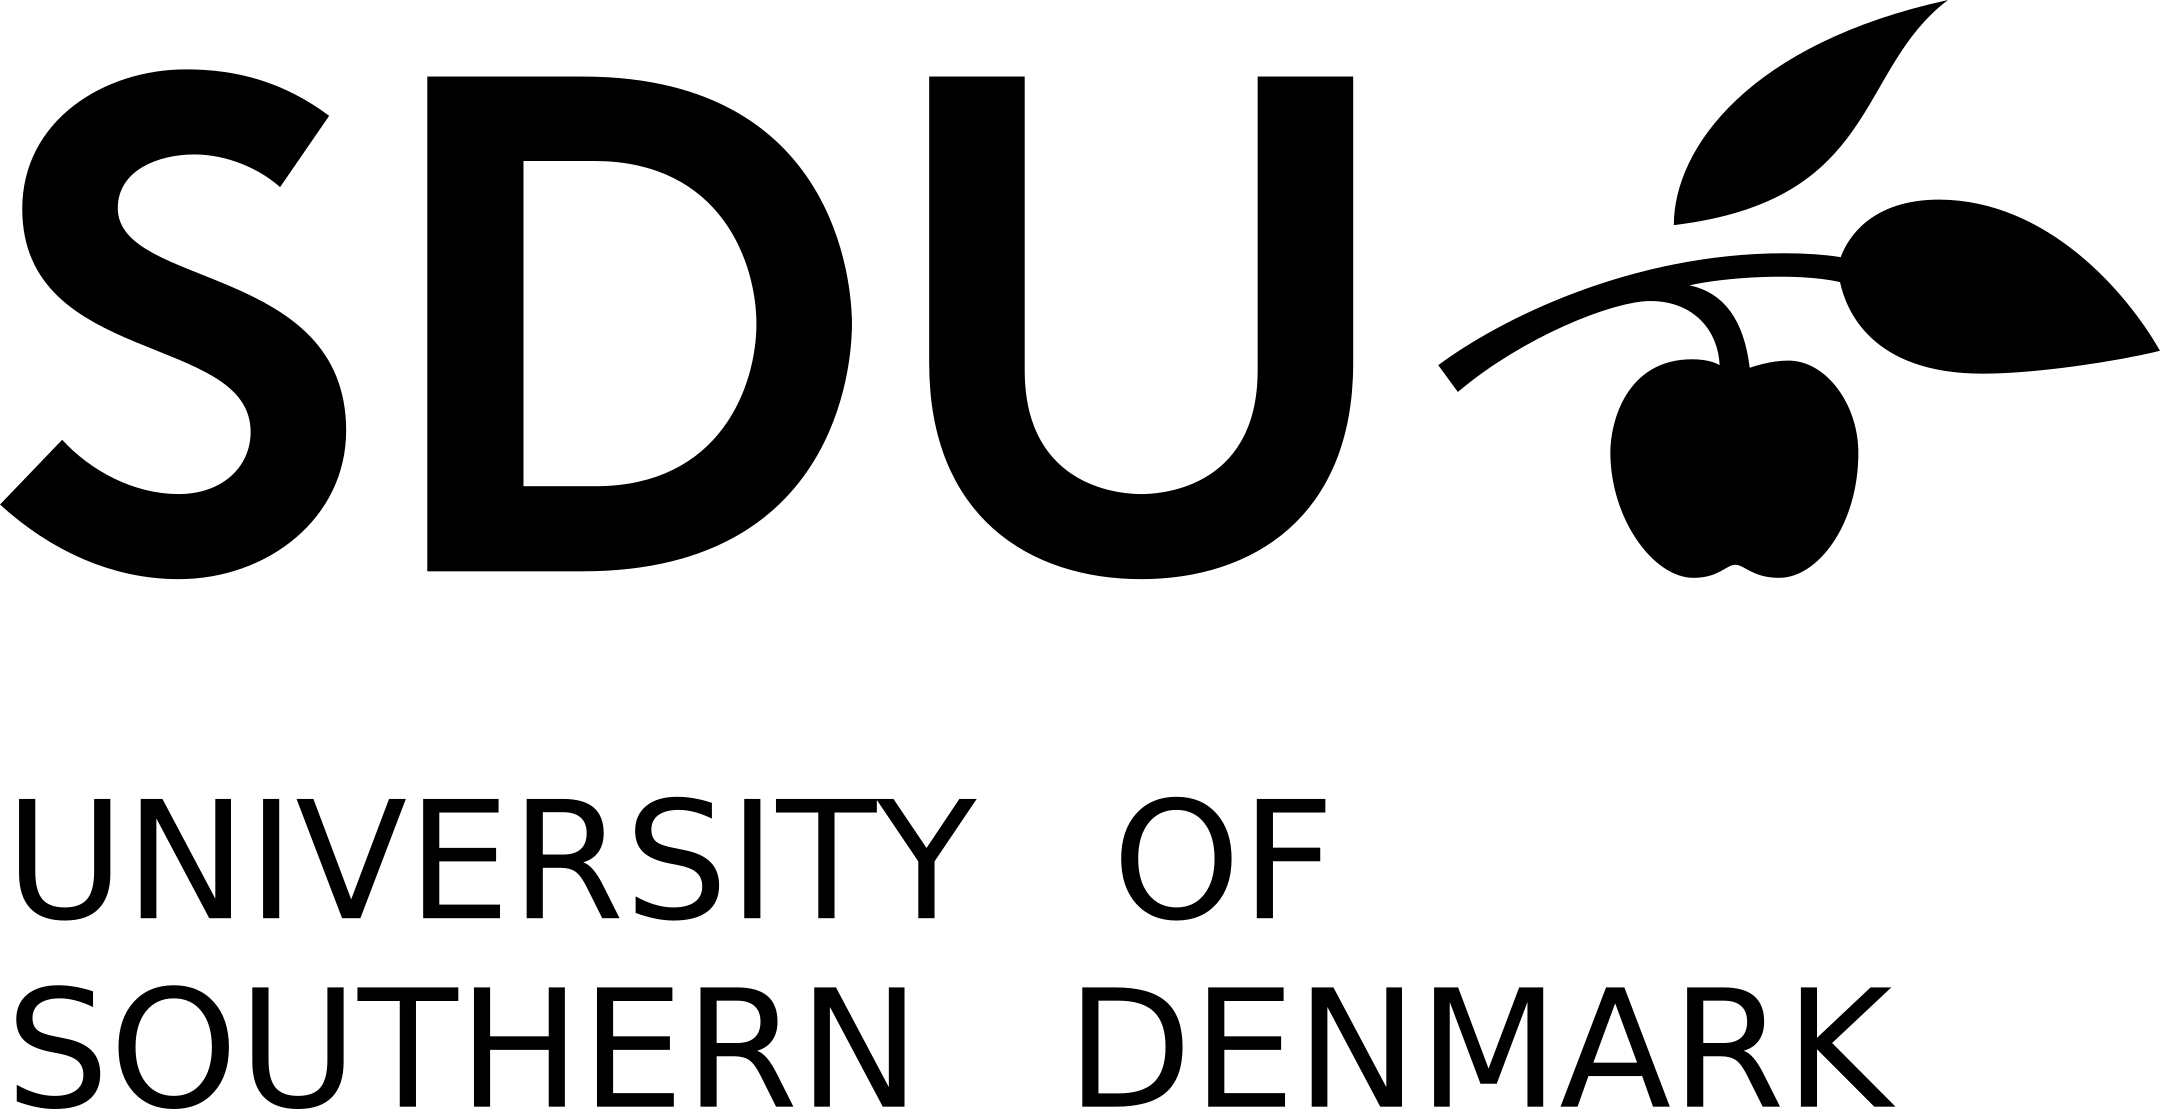
\includegraphics[scale=1]{../SDU_logo.png}
    \vfill\ 
    \vspace{5mm}
    IMADA \\

    \textbf{\datedate} \\[2\baselineskip]
\end{titlepage}

\renewcommand{\thepage}{\roman{page}}% Roman numerals for page counter
\tableofcontents
\newpage
\setcounter{page}{1}
\renewcommand{\thepage}{\arabic{page}}

\part{Formal course description}

\section{Aim}
Machine learning has become a part in our everydays life, from simple product recommendations to personal electronic assistant to self-driving cars. More recently, through the advent of potent hardware and cheap computational power, “Deep Learning” has become a popular and powerful tool for learning from complex, large-scale data.
In this course, we will discuss the fundamentals of deep learning and its application to various different fields. We will learn about the power but also the limitations of these deep neural networks. At the end of the course, the students will have significant familiarity with the subject and will be able to apply the learned techniques to a broad range of different fields.\\
\vspace{10mm}

The course builds partly on the knowledge acquired in the course DM555 but can be taken by any Computer Science or Computational BioMedicine Master student.\\
\vspace{10mm}

In relation to the competence profile of the degree it is the explicit focus of the course to:
\begin{itemize}
\item giving the competence to plan and execute a deep learning task by means of deep neural networks.
\item providing knowledge on the different types of deep learning approaches including their advantages and disadvantages.
\item transfer learned methods to new fields of applications.
\item challenges the student with real-life datasets and problem-solving skills
\end{itemize}

\section{Statement of aims}
\begin{itemize}
\item The learning objectives of the course is that the student demonstrates the ability to:
\item Describe the principles of deep neural networks in a scientific and precise language and notation
\item Analyze the various types of neural networks, the different layers and their interplay 
\item Describe the feasibility of deep learning approaches to concrete problems
\item Understand the theoretical mathematical foundations of the field 
\item Apply deep learning frameworks for solving concrete problems
\end{itemize}


\section{Pensum}

\begin{itemize}
\item All lecture slides are relevant for the exams.
\item All readings noted in the lecture list are relevant for the exam.
\item Ian Goodfellow, Yoshua Bengio, Aaron Courville - The Deep Learning Book
\item Gareth James, Daniela Witten, Trevor Hastie - Robert Tibshirani An Introduction to Statistical Learning (ISL)

\end{itemize}


\part{exam topics}

\section{Exam Form}

5 minute presentation from the 6 topics\\
10 minutes questions

\newpage
\section{Feed-Forward Networks}

\subsection{introduction}

\subsection{Function Principle}
\subsection{Output Units}
\subsection{Hidden Units}
...



\newpage
\section{Backpropagation}

\subsection{introduction}
\subsection{Function Principle}
\subsection{Computational Graphs}
\subsection{Backpropagation through time}
...


\newpage
\section{Regularization}
\subsection{introduction}
\subsection{Over/Underfitting \& Model Capacity}
\subsection{Parameter Penalties}
\subsection{Bagging}
\subsection{Dropout}
...

\newpage
\section{Convolutional Neural Networks}
\subsection{introduction}
\subsection{Function Principle}
\subsection{Pooling}
\subsection{Initialization of the kernels}
...

\newpage
\section{Recurrent Neural Networks}
\subsection{introduction}
\subsection{Function Principle}
\subsection{Problems with long term memory}
\subsection{Long Short Term Memory}
...

\newpage
\section{Optimization for Neural Networks}
\subsection{introduction}
\subsection{Parameter Initialization}
\subsection{Adaptive Learning}
\subsection{Batch Normalization}
\subsection{Pre-training}
...

\newpage
\section{Autoencoders and GANs}
\subsection{introduction}
\subsection{Autoencoders}
\subsection{Variational Autoencoders}
\subsection{GANs}
...

\end{document}